\subsection{Grobkonzept}
\label{sec:Grobkonzept}

Das Ziel einer möglichst ansprechenden, visuellen Darstellung des
Studienstandorts Lingen und des neuen Campus unter Verwendung moderner
Webtechnologien lässt sich auf verschiedenste Weisen realisieren. 

In einem Ideenfindungsprozess hat die Projektgruppe für die Erreichung der
Projektziele geeignete Umsetzungsmöglichkeiten identifiziert. Mit der
Brainstorming-Methode wurden zunächst sämtliche Ideen zur Realisierung der
Projektidee gesammelt. Die Ideensammlung, die auf diese Weise entstand, wurde
anschließend gefiltert und sortiert. Die einzelnen Ideen wurden zu Clustern, wie
beispielsweise "`Anforderungen aus dem Zielsystem"', "`Technologien"' und
"`Funktionalität des Systems"' zusammengefasst. Anhand dieser strukturierten
Ideensammlung wurden dann konkrete Möglichkeiten zur Umsetzung der Projektidee
herausgearbeitet. Nach einer ersten Filterung der Umsetzungsmöglichkeiten hat
sich die Projektgruppe auf die folgenden drei Realiserungsalternativen geeinigt. 
% TODO: Evtl. weiter Untersuchung

% Konkret hat die Projektgruppe folgende Alternativen im Zuge der Ideenfindung
% herausgestellt:

\begin{description}
\item[Fotogalerie] \hfill \\
Innerhalb einer Fotogalerie soll dem Anwender der modernisierte Studienstandort
Lingen näher gebracht werden. Zu den Fotos könnten entsprechende
Informationstexte, Beschreibungen und weiterführende Links für
Studieninteressierte hinterlegt werden.
\item[Virtueller Rundgang im Stile von Google Street View] \hfill \\
Der Anwender soll interaktiv durch Panoramafotos von den Räumlichkeiten des
Campus navigieren können. Auch bei dieser Möglichkeit der Projektrealisierung
könnten dem Nutzer weiterführende Informationen zu den abgebildeten Inhalten
präsentiert werden.
\item[Virtueller Rundgang durch ein 3D-Modell] \hfill \\
Bei dieser Möglichkeit der Umsetzug soll ein 3D-Modell des gesamten
Campusgebäudes erstellt werden. Der Nutzer könnte dann virtuell duch die
modellierten Räumlichkeiten des Campus navigieren und auf diese Weise einen
Eindruck vom Studienstandort erlangen.
\end{description}

Hierbei unterscheiden sich die einzelnen Alternativen in Innovativität,
Attraktivität für den Anwender, Komplexität der Umsetzung und Grad der Zielerreichung voneinander.
Die folgende \tabelle{AlternativenVergleich} stellt die drei Varianten
hinsichtlicher der vier genannten Kritierien gegenüber.

\begin{table}[h]
\centering
\begin{tabular}{ccccl}
\hline
\multicolumn{1}{l}{}              & Innovativität & Attraktivität & Komplexität & Grad der Zielerreichung \\ \hline
Fotogalerie                       & gering        & mittel        & gering      & gering                  \\ \hline
Virtueller 3D Rundgang            & hoch          & hoch          & sehr hoch   & hoch                    \\ \hline
Google Street View Rundgang       & hoch          & hoch          & hoch        & hoch                    \\ \hline
\end{tabular}
\caption{Soll-Ist-Vergleich der Kostenplanung}%
\label{tab:AlternativenVergleich}%
\end{table}

Die vorangegangene Tabelle verdeutlicht, dass die Komplexität des virtuellen Rundgangs und der 3D-Modellierung gegenüber 
der Fotogalerie höher ist. Der Grund dafür ist, dass für diese beiden Lösungsansätze Einarbeitungsaufwand notwendig ist. 
Dieser Aufwand fällt bei der Fotogalerie nicht an, da es sich hier nur um eine vorhandene Fotogalerie handelt, welche 
lediglich um statische Bilder ergänzt werden soll. Dadurch resultiert auch der geringe Grad der Zielerreichung bei der 
Umsetzung mit der Fotogalerie, da die Informationsdarstellung bei statischen Fotos nicht so komplex gestaltet werden kann 
wie bei den beiden anderen Lösungsansätzen.

% Die Projektgruppe geht davon aus, dass vielen Nutzern innerhalb der Zielgruppe
% diese Darstellungsform durch Google Street View bereits bekannt ist. Um von den
% vorhandenen Erfahrungen der Nutzer profitieren zu können sollen bekannten
% Steuerungselemente von Google Street View adaptiert werden. Diese sind in
% \abbildung{GoogleStreetView} dargestellt.

% \begin{figure}[htb] 
% \centering
% 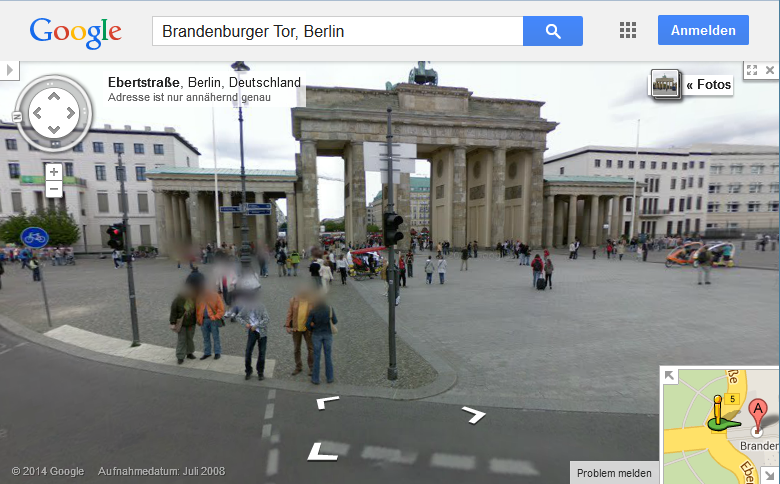
\includegraphics[width=0.7\textwidth]{GoogleStreetView.png}
% \caption[Google Street View]{Google Street View\protect\footnotemark}
% \label{fig:GoogleStreetView}
% \end{figure}
% \footnotetext{Screenshot von \url{https://maps.google.de/}}

% Die Realisierung der Projektziele wäre nach einer ersten Einschätzung der
% Projektmitglieder mit jeder der dei vorgestellten Umsetzungsmöglichkeiten
% vorstellbar. Im weiteren Verlauf der Konzeptionierungsphase soll jedoch die
% Möglichkeit herausgestellt werden, welche der Möglichkeiten für die
% Erreichung der Projektziele am besten geeignet ist.
